\documentclass{article}
\usepackage{CJK}
\usepackage{amsmath}
\usepackage{amsthm}
\usepackage{amsfonts}
\usepackage{palatino}
\usepackage{xcolor}
\usepackage{geometry}
\usepackage{listings}
\usepackage{pxfonts}
\usepackage{enumerate}
\usepackage[pdftex]{graphicx}
\geometry{left=2cm,right=2cm,top=3cm,bottom=3cm}
\pagestyle{myheadings}
\markright{Huiqian Yu/14300180118}
\setlength{\parindent}{0pt}
\newcommand{\ix}[1]{\intertext{{}#1}}
\newcommand{\dx}{\;\mathrm{d}\,x}
\newcommand{\dt}{\;\mathrm{d}\,t}
\newcommand{\dm}[1]{\;\mathrm{d}\,{}#1}
\newcommand{\ve}{\varepsilon}
\newcommand{\tp}{^\mathsf{T}}
\newcommand{\var}{\mathrm{var}}
\newcommand{\corr}{\mathrm{corr}}
\newcommand{\mbe}[1]{\mathbb{E}\left[{}#1\right]}
\newcommand{\argmin}[1]{\mathop{\arg\min}_{{}#1}}
\newcommand{\suml}[3]{\sum\limits_{#1=#2}^{#3}}
\newcommand{\e}{\mathrm{e}}
\newcommand{\vari}{\mathrm{i}}
\definecolor{backcolour}{rgb}{0.95,0.95,0.92}
\begin{document}
\begin{CJK*}{GBK}{song}

\section*{Problem 1}
\subsection*{4.6}
\subsubsection*{(a)}
\begin{align*}
	\gamma(0)&=\var(s_t)+A^2\var(s_t)+2A\gamma_s(D)+\var(n_t)\\
	\int_{-1/2}^{1/2}f_x(\omega)\dm \omega&=
	\int_{-1/2}^{1/2}(1+A^2)f_s(\omega)+f_n(\omega)+f_s(\omega)\e^{2\pi \vari \omega D}\dm \omega\\
	&=\int_{-1/2}^{1/2}(1+A^2+2A\cos(2\pi\omega D))f_s(\omega)+f_n(\omega)\dm \omega
\ix{Thus,}
	f_x(\omega)&=(1+A^2+2A\cos(2\pi\omega D))f_s(\omega)+f_n(\omega)
\end{align*}
\subsubsection*{(b)}
Observe the periodically change in $f_x(\omega)$. Besides the period of $f_s(\omega)$, there should be another period of $1/D$.
\subsection*{4.8}
\begin{lstlisting}[language=R,keywordstyle=\color{blue!70},commentstyle=\color{red!50!green!50!blue!50},frame=single,rulesepcolor=\color{red!20!green!20!blue!20},backgroundcolor=\color{backcolour},
]
library(astsa)
ss = sunspotz
ss.per = spec.pgram(sunspotz, taper = 0, log = 'no', detrend = T)
abline(v = 1/10, lty = 'dotted')
abline(v = 22/240, lty = 'dotted')

U = qchisq(0.025,2)
L = qchisq(1 - 0.025,2)

# Output
> ss.per$spec[24]
[1] 30583.29
> 2*ss.per$spec[22]/L
[1] 8804.265
> 2*ss.per$spec[22]/U
[1] 1282807
> 2*ss.per$spec[24]/L
[1] 8290.672
> 2*ss.per$spec[24]/U
[1] 1207975
\end{lstlisting}
\newpage
The periodogram is shown below.
\begin{center}
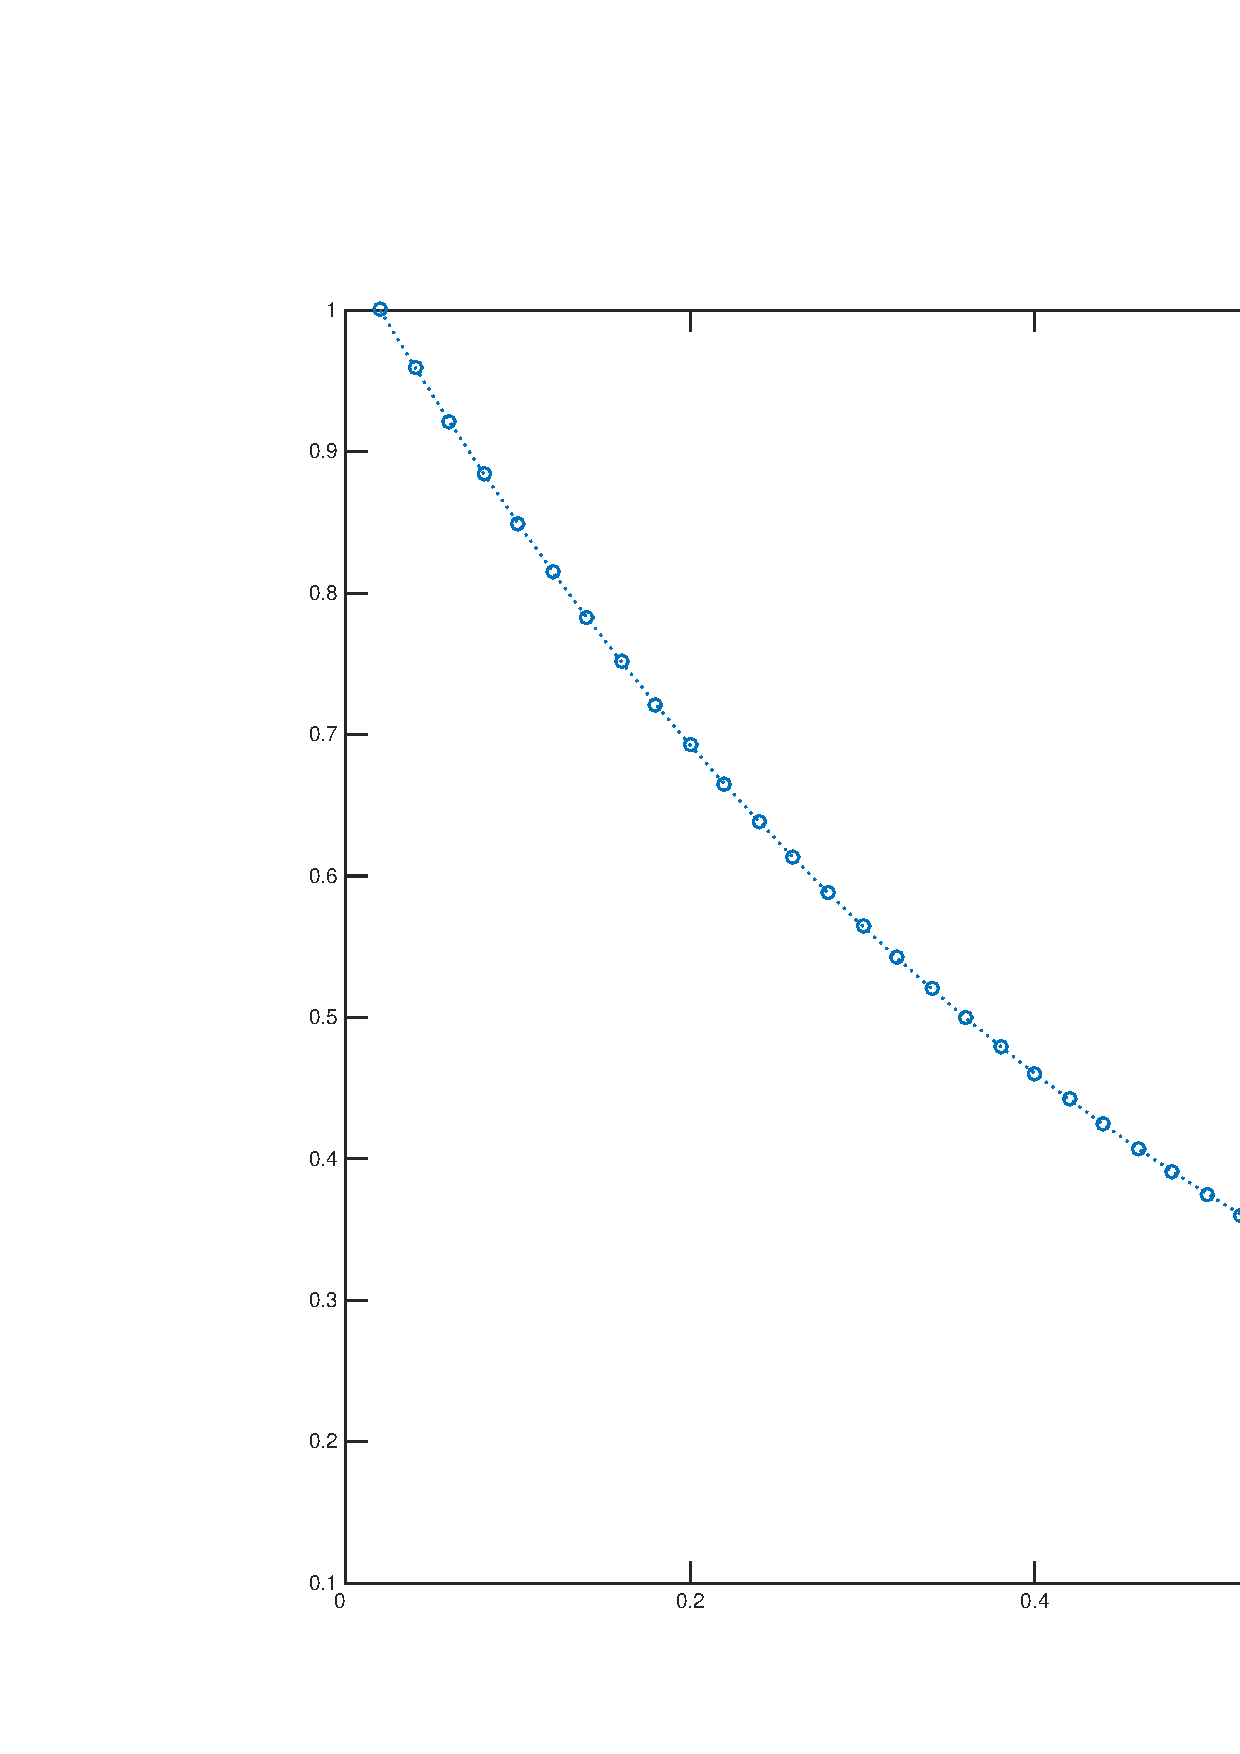
\includegraphics[width=12cm]{1.png}
\end{center}
The result shows that the periodogram as an estimator is susceptible to large uncertainties.
\subsection*{4.9}
\begin{lstlisting}[language=R,keywordstyle=\color{blue!70},commentstyle=\color{red!50!green!50!blue!50},frame=single,rulesepcolor=\color{red!20!green!20!blue!20},backgroundcolor=\color{backcolour},
]
library(astsa)

par(mfrow=c(2,1))
plot(salt)
plot(saltemp)

par(mfrow=c(2,1))
salt.per = spec.pgram(salt, taper = 0, log = 'no', detrend = T)
abline(v = 1/16, lty = 'dotted')
saltemp.per = spec.pgram(saltemp, taper = 0, log = 'no', detrend = T)
abline(v = 1/16, lty = 'dotted')

> salt.per$spec[4]
[1] 60.66648
> saltemp.per$spec[4]
[1] 2.43787
U = qchisq(0.025,2)
L = qchisq(1 - 0.025,2)
> 2*salt.per$spec[4]/L
[1] 16.44577
> 2*salt.per$spec[4]/U
[1] 2396.198
> 
> 2*saltemp.per$spec[4]/L
[1] 0.6608701
> 2*saltemp.per$spec[4]/U
[1] 96.29072
\end{lstlisting}
It's shown that the level of salt is corresponding to the average tempearture for the soil.
\begin{center}
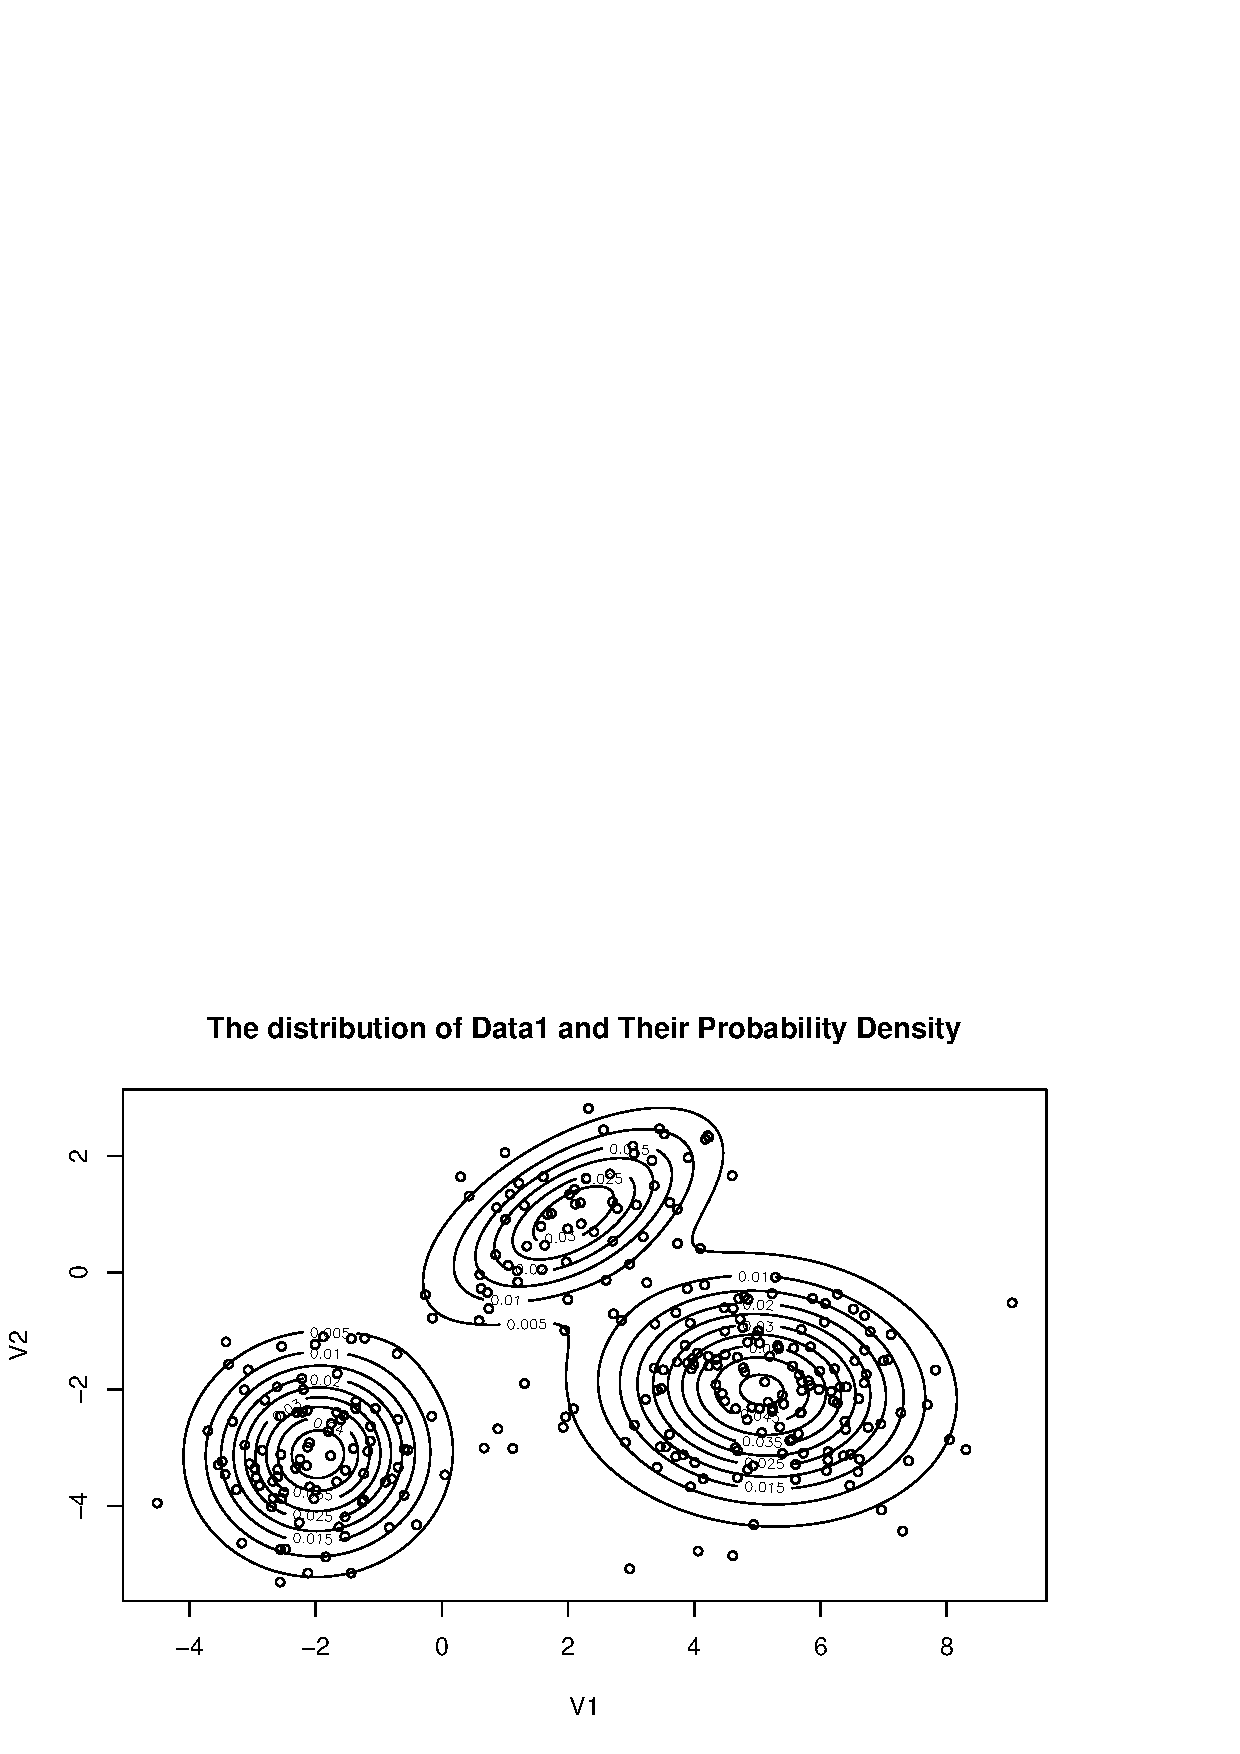
\includegraphics[width=10cm]{2.png}
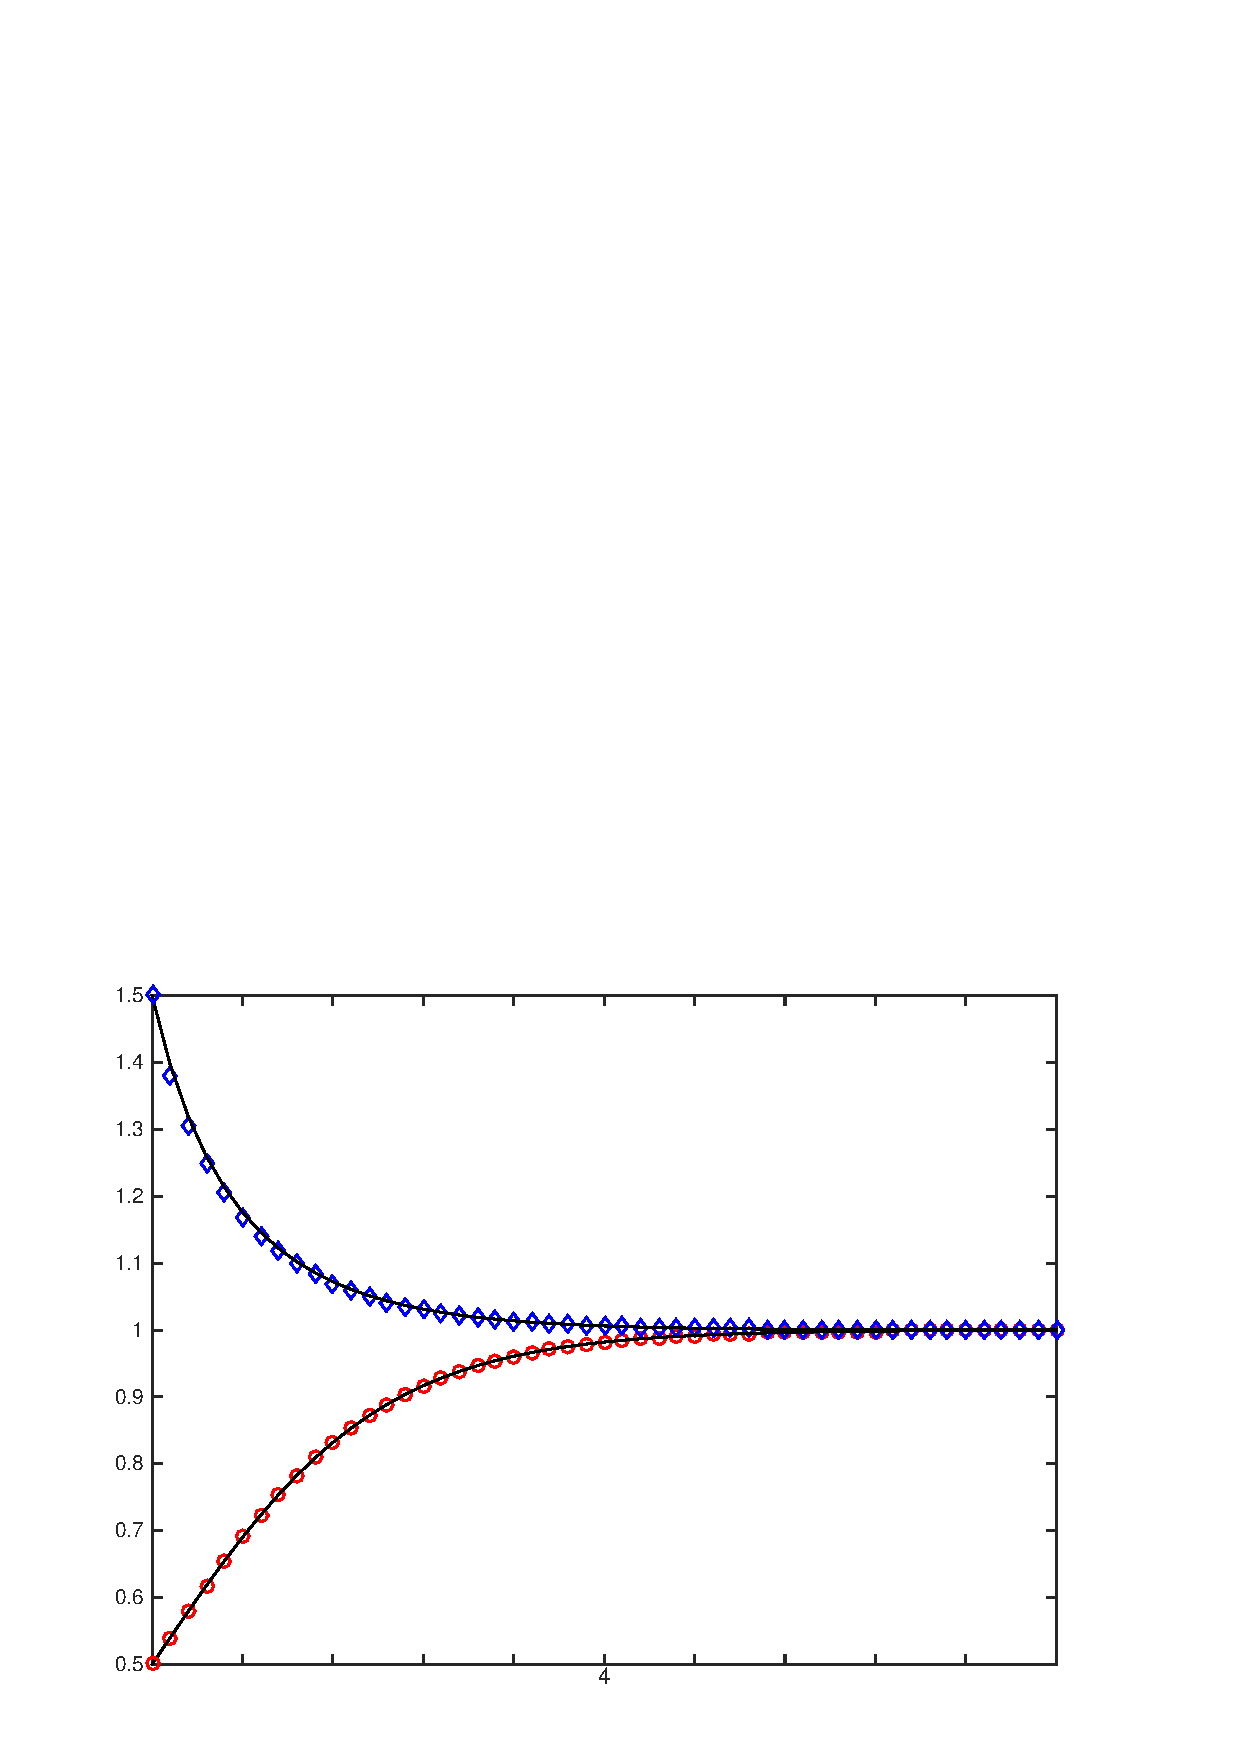
\includegraphics[width=10cm]{3.png}
\end{center}

\section*{Problem 2}
\begin{align*}
\ix{\bf(a)\rm}
\ix{Since $\gamma(h)$ is non-negative definite, define}
	f_n(\omega)&=\dfrac 1n \suml s1n \suml t1n \exp(-2\pi \vari\omega s)\gamma(r-s)\exp (2\pi\vari\omega r)\\
	&=\dfrac 1n \suml h{-(n-1)}{n-1}(n-|h|)\exp(-2\pi\vari\omega h)\gamma(h)\ge 0
\ix{Since $\gamma(h)$ is absolutely summable,}
	f(\omega)&=\lim\limits_{n\rightarrow \infty}f_n(\omega)\\
	&=\suml h{-\infty}\infty \gamma(h)\exp(-2\pi\vari\omega h)\ge 0
\ix{\bf(b)\&(c)\rm}
\ix{Since $\gamma(h) = \gamma(-h)$,}
	f(\omega)&=\suml h{-\infty}\infty \gamma(h)\exp(-2\pi\vari\omega h)\\
	&= \gamma(0) + 2\suml h1\infty \gamma(h)\cos(2\pi\omega h)
\ix{Thus,}
	f(-\omega)&=\gamma(0)+2\suml h1\infty \gamma(-h)\cos(-2\pi\omega h)=f(\omega)\\
	f(1-\omega)&=\gamma(0) + 2\suml h1\infty \gamma(h)\cos(2\pi h-2\pi\omega h)=f(\omega)
\ix{\bf(d)\rm}
	\int_{-1/2}^{1/2}\exp(2\pi\vari\omega h)f(\omega)\dm \omega&=\int_{-1/2}^{1/2}\suml k{-\infty}\infty \gamma(h)\exp(-2\pi\vari\omega (h-k))\dm \omega\\
	&=\suml k{-\infty}\infty\int_{-1/2}^{1/2}\gamma(h)\exp(-2\pi\vari\omega (h-k))\dm \omega
\ix{if $k\ne h$, $\int_{-1/2}^{1/2}\gamma(h)\exp(-2\pi\vari\omega (h-k))\dm \omega = 0$, so}
	\int_{-1/2}^{1/2}\exp(2\pi\vari\omega h)f(\omega)\dm \omega&=\int_{-1/2}^{1/2}\gamma(h)\dm \omega\\
	&=\gamma(h)
\end{align*}

\end{CJK*}
\end{document}
